% chapter02.tex

 %%%%%%%%%%%%%%%%%%%%%%%%%%%%%%%%%%%%%%%%%%%%%%%%%%%%%%%%%%%%%%%%%%%%%%%%%%%%%
 %                                                                           %
 %    PyMS documentation                                                     %
 %    Copyright (C) 2005-8 Vladimir Likic                                    %
 %                                                                           %
 %    The files in this directory provided under the Creative Commons        %
 %    Attribution-NonCommercial-NoDerivs 2.1 Australia license               %
 %    http://creativecommons.org/licenses/by-nc-nd/2.1/au/                   %
 %    See the file license.txt                                               %
 %                                                                           %
 %%%%%%%%%%%%%%%%%%%%%%%%%%%%%%%%%%%%%%%%%%%%%%%%%%%%%%%%%%%%%%%%%%%%%%%%%%%%%

\chapter{Peak lists and GC-MS experiments}

\section{Introduction}

This chapter demonstrates main functions of PyMS in a tutorial like manner.
The data files used in the examples are provided in the project 'pyms-data'.
The commands executed interactively are grouped together by example, and
provided as Python scripts in the project 'pyms-test'.

The setup used in the examples below is as follows. The projects 'pyms',
'pyms-test', 'pyms-docs', and 'pyms-data' were downloaded in the directory
{\tt /home/current/proj/PyMS}. In the project 'pyms-test' there is a directory
corresponding to each example coded with the example number (ie.
{\tt pyms-test/01/} corresponds to Example 1). In each example directory
there is a script named 'proc.py' which contains the commands given in
the example. Provided that the paths to 'pyms' and 'pyms-data' are set
properly, these scripts could be run with the following command:

\begin{verbatim}
$ python proc.py
\end{verbatim}

Before running each example the Python interpreter was made aware of the
PyMS location with the following commands:

\begin{verbatim}
import sys
sys.path.append("/home/current/proj/PyMS/")
\end{verbatim}

For brevity these commands will not be shown in the examples below, but
they are included in 'pyms-test' example scripts.  The above path need
to be adjusted to match your own location of pyms.

All data files (raw data files, peak lists etc) used in the example below
can be found in 'pyms-data'.


\section{Reading of GC-MS data and basic manipulation of data}

\subsection{Reading ChemStation GC-MS data into PyMS}

\noindent
[ {\em This example is in pyms-test/01} ]

The PyMS package pyms.IO provides capabilities to read the raw GC-MS
data stored in the ANDI-MS format. The function IO.ANDI.ChemStation()
provides the interface to ANDI-MS data files saved from Agilent
ChemStation software.\footnote{ANDI-MS data format stands for Analytical
Data Interchange for Mass Spectrometry, and was developed for the
description of mass spectrometric data developed in 1994 by Analytical
Instrument Association. ANDI-MS is essentially a recommendation, and
it is up to individual vendors of mass spectrometry processing software
to implement "export to ANDI-MS" feature in their software.}

The file 'a0806\_140.CDF' is a GC-MS experiment exported from Agilent
ChemStation (located in 'pyms-data'). This file can be loaded in the
memory as follows:

\begin{verbatim}
>>> from pyms.IO.ANDI.Class import ChemStation
>>> andi_file = "/home/current/proj/PyMS/pyms-data/a0806_140.CDF"
>>> andi_data = ChemStation(andi_file)
 -> Processing netCDF file '/home/current/proj/PyMS/pyms-data/a0806_140.CDF'
    [ 3236 scans, masses from 50 to 550 ]
>>>
\end{verbatim}

\noindent
The above command creates the object 'andi\_data' which is an {\em instance}
of the class IO.ANDI.ChemStation.

\subsection{Exploring an ANDI-MS data object}

The object 'andi\_data' has several attributes and methods associated with it.

\begin{verbatim}
>>> print "ANDI-MS data filename:", andi_data.get_filename()
ANDI-MS data filename: /home/current/proj/PyMS/pyms-data/a0806_140.CDF
\end{verbatim}

The method {\tt get\_tic()} return total ion chromatogram (TIC) of the data
as an IonChromatogram object:

\begin{verbatim}
tic = andi_data.get_tic()
\end{verbatim}

\noindent
An IonChromatogram object is a one dimensional vector containing
mass intensities as a function of retention time. This can can be either
m/z channel intensities (for example, ion chromatograms at m/z = 65),
or cumulative intensities over all measured m/z (TIC).

The method {\tt get\_ic\_at\_index(i)} returns i-th ion chromatogram, as
an IonChromatogram object. For example, to get the first ion chromatogram
from the data:

\begin{verbatim}
ic = andi_data.get_ic_at_index(1)
\end{verbatim}

The method {\tt get\_ic\_at\_mass(MZ)} returns the ion chromatogram for
m/z = MZ.  For example, to get the ion chromatogram that corresponds
to m/z = 73:

An ion chromatogram object has a method {\tt is\_tic()} which returns
True is the ion chromatogram is TIC, False otherwise:

\begin{verbatim}
>>> print "'tic' is a TIC:", tic.is_tic()
'tic' is a TIC: True
>>> print "'ic' is a TIC:",ic.is_tic()
'ic' is a TIC: False
\end{verbatim}

\subsection{Writing data to a file}

The method {\tt write()} of IonChromatogram object allows one to save
the ion chromatogram object to a file:

\begin{verbatim}
>>> tic.write("output/tic.dat", minutes=True)
>>> ic.write("output/ic.dat", minutes=True)
\end{verbatim}

\noindent
The flag minutes=True indicates that retention time will be saved in minutes.
The ion chromatogram object saved with with the {\tt write{}} method is a
plain ASCII file which contains a pair of (retention time, intensity) per
line:

\begin{verbatim}
$ head tic.dat
  5.0944      745997.0000
  5.1002      726566.0000
  5.1059      717704.0000
  5.1116      684214.0000
  5.1173      701866.0000
  5.1230      893306.0000
  5.1287     1278099.0000
  5.1345     1290984.0000
  5.1402      925558.0000
  5.1459      644122.0000
\end{verbatim}

\noindent
Figure \ref{fig:tic-plot} shows the plot of the file 'tic.dat' produced with the
program Gnuplot. The Gnuplot script used to produce this plot is provided
as pyms-test/01/output/plot.gnu.

\begin{figure}[htp]
\begin{center}
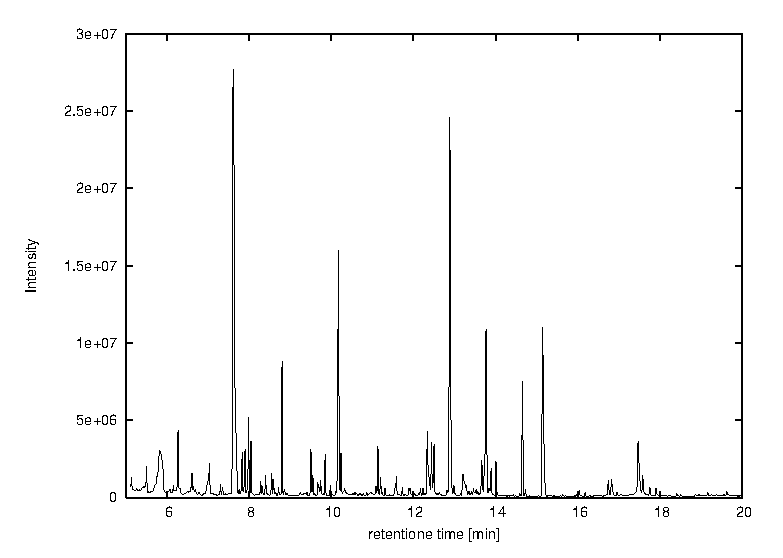
\includegraphics{graphics/pyms-test/tic.eps}
\caption{The Gnuplot plot of the file 'tic.dat'}
\label{fig:tic-plot}
\end{center}
\end{figure}

The method {\tt get\_intensity\_matrix()} of ChemStation object returns
the entire matrix of intensities:

\begin{verbatim}
>>> im = andi_data.get_intensity_matrix()
>>> print "Dimensions of the intensity matrix are:",len(im),"x",len(im[0])
Dimensions of the intensity matrix are: 3236 x 501
\end{verbatim}

\noindent
This data matrix contains 3236 time points (MS scans), and each time point
corresponds to a mass spectrum of 501 m/z points.

The intensity matrix can be saved to a file with the function 'save\_data()':

\begin{verbatim}
save_data("output/im.dat", im)
\end{verbatim}

The entire data (ie. ChemStation object) can be saved as CSV with the method
{\tt export\_csv()}. For example,

\begin{verbatim}
>>> andi_data.export_csv("output/data")
\end{verbatim}

\noindent
will create 'data.im.csv, data.mz.csv, and data.rt.csv where these are the
intensity matrix, retention time vector, and m/z vector in the CSV format.

\subsection{Reading Xcalibur GC-MS data into PyMS}

\noindent
[ {\em This example is in pyms-test/01a} ]

The function IO.ANDI.Xcalibur() provides the interface to ANDI-MS data files
exported from Thermo Scientific Xcalibur software.\footnote{Due to differences
in the interpretation of the ANDI-MS format PyMS implements separate parsers
for different software packages}

The file '121107B\_10.CDF' is a GC-MS experiment exported from Xcalibur (located
in 'pyms-data'). This file can be loaded as follows:

\begin{verbatim}
>>> from pyms.IO.ANDI.Class import Xcalibur
>>> andi_file = "/home/current/proj/PyMS/pyms-data/121107B_10.CDF"
>>> andi_data = Xcalibur(andi_file)
 -> Processing netCDF file '/home/current/proj/PyMS/pyms-data/121107B_10.CDF'
    [ 7038 scans, masses from 70 to 600 ]
>>>
\end{verbatim}

\noindent
The above command creates the object 'andi\_data' which is an {\em instance}
of the class IO.ANDI.Xcalibur. IO.ANDI.ChemStation and IO.ANDI.Xcalibur 
inherit attributes and methods from the class IO.ANDI.ANDIMS\_reader
(a generic ANDI-MS parser) and thus provide the same functionality.

\section{Creating signal peaks}

\noindent
[ {\em This example is in pyms-test/02} ]

In PyMS a signal peak is represented as 'Peak' object defined in
pyms.Peak.Class.py. A peak object is initialized with two arguments:
peak retention time and peak raw area. The following commands create
a peak named 'p' with the retention time of 7.311 min and a peak area
of 33768615 (this is the peak no. 36 in the ChemStation peak area report
file 'a0806\_140.txt'):

\begin{verbatim}
>>> from pyms.Peak.Class import Peak
>>> p = Peak(7.311*60.0,33768615)
\end{verbatim}

\noindent
As a matter of convention PyMS internally stores retention times in seconds,
hence above the retention time is multiplied by 60. Peak raw area is in
arbitrary units.

\begin{figure}[htp]
\begin{center}
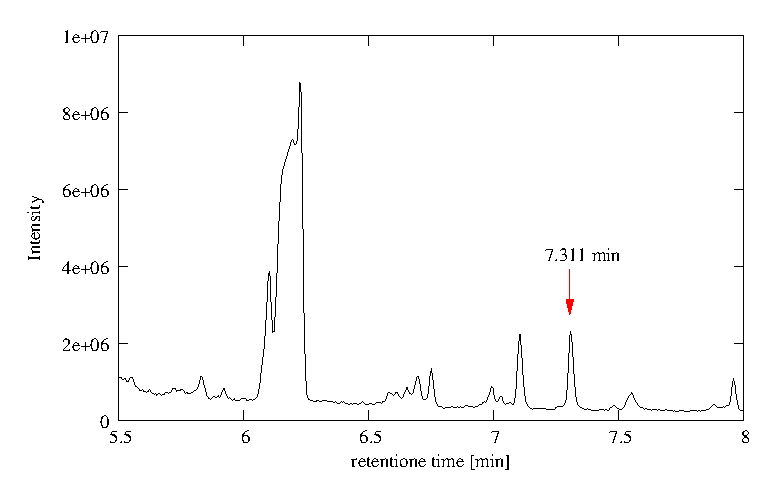
\includegraphics{graphics/tic_with_peak/tic_with_peak.eps}
\caption{The TIC calculated from the data file 'a0806\_140.CDF', plot showing the
segment with retention times 5.5 to 8.0 minutes. The annotation shows the peak at
7.311 minutes.}
\label{fig:mass-spectrum}
\end{center}
\end{figure}

Peak properties can be accessed through its attributes:

\begin{verbatim}
>>> print "Peak retention time is", p.rt
Peak retention time is 438.66
>>> print "Peak raw area is", p.raw_area
Peak raw area is 33768615.0
\end{verbatim}

\noindent
Other important properties of a peak object are peak normalized area
and peak mass spectrum. The peak created in the above example does
not have values associated with these two attributes, and they are
merely initialized to 'None':

\begin{verbatim}
>>> print "Peak normalized area is", p.norm_area
Peak normalized area is None
>>> print "Peak mass spectrum is", p.mass_spectrum
Peak mass spectrum is None
\end{verbatim}

\noindent
The peak mass spectrum can be set by calling the method {\tt set\_mass\_spectrum()}.
We first need to load the raw data,

\begin{verbatim}
>>> andi_file = "/home/current/proj/PyMS/pyms-data/a0806_140.CDF"
>>> andi_data = ChemStation(andi_file)
>>> p.set_mass_spectrum(andi_data)
\end{verbatim}

\noindent
This will set the mass spectrum attribute: 

\begin{verbatim}
>>> print p.mass_spectrum
[     0  28072  48376   6975   1163   3369   3569   4740  26872  16560
   2742   5956    790    838    625    684   1144   1367   1015   8214
   6023   1342   3325 241024  27744  56136   6238   3281  11883  67456
[--output deleted--]
\end{verbatim}

\noindent
These are m/z channel intensities in arbitrary units. The m/z values
themselves are in the mass list attribute:

\begin{verbatim}
>>> print p.mass_list
[50, 51, 52, 53, 54, 55, 56, 57, 58, 59, 60, 61, 62, 63, 64, 65,
66, 67, 68, 69, 70, 71, 72, 73, 74, 75, 76, 77, 78, 79, 80, 81,
82, 83, 84, 85, 86, 87, 88, 89, 90, 91, 92, 93, 94, 95, 96, 97,
[--outout deleted--]
\end{verbatim}

\noindent
The m/z values go from 50 to 550 (a total of 501 values).  The length of
the two arrays must match:

\begin{verbatim}
>>> print len(p.mass_spectrum)
501
>>> print len(p.mass_list)
501
\end{verbatim}

The mass spectrum can be written to a file by calling the peak
{\tt write\_mass\_spectum()} method:

\begin{verbatim}
>>> p.write_mass_spectrum("output/ms.dat")
\end{verbatim}

\noindent
The file 'output/ms.dat' contains the pairs (mz, intensity), one pair
per line:

\begin{verbatim}
$ head output/ms.dat
  50.000            0.000
  51.000        28072.000
  52.000        48376.000
  53.000         6975.000
  54.000         1163.000
  55.000         3369.000
  56.000         3569.000
  57.000         4740.000
  58.000        26872.000
  59.000        16560.000
\end{verbatim}

Figure \ref{fig:mass-spectrum} shows the plot of ms.dat created with the
program Gnuplot.

\begin{figure}[htp]
\begin{center}
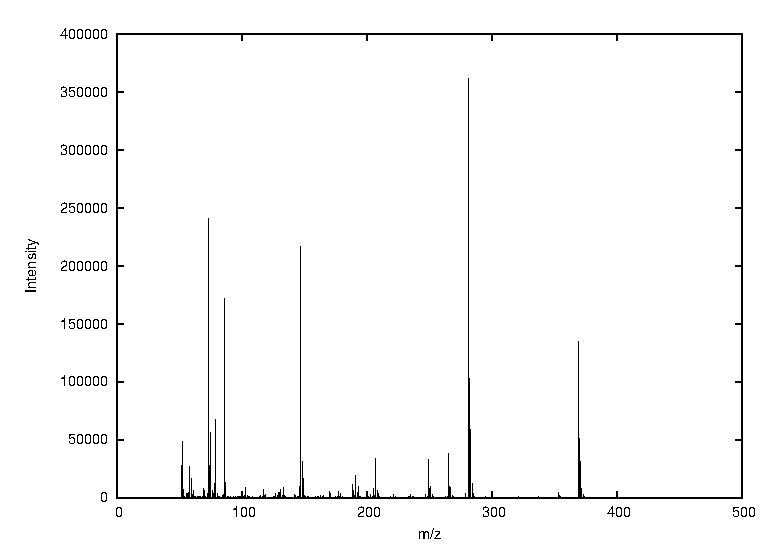
\includegraphics{graphics/pyms-test/ms.eps}
\caption{The mass spectrum of the peak at 7.311 min. The mass spectrum was
saved to a file 'ms.dat', and the plot was produced with the gnuplot script
file 'pyms-test/02/output/plot.gnu'.}
\label{fig:mass-spectrum}
\end{center}
\end{figure}

\section{Creating an experiment from ChemStation data}

\noindent
[ {\em This example is in pyms-test/03} ]

The input files used in this example are 'a0806\_140.CDF' (ANDI-MS data
file exported from Agilent ChemStation) and 'a0806\_140.txt.a' (the 
corresponding peak area report file generated by ChemStation).

The original peak area report file exported from ChemStation is
'a0806\_140.txt'. This file was manually edited to flag non-informative
peaks, and also peaks which originate from internal reference compounds
added during the sample preparation. For example, below is the snippet
of the original file 'a0806\_140.txt':

\begin{verbatim}
 52   8.215   470  478  480 PV 3   91906   1414873   0.14%   0.056%
 53   8.242   480  483  486 VV 4   99010   1301807   0.13%   0.051%
 54   8.285   486  490  495 VV 2  124626   2241940   0.22%   0.088%
 55   8.337   495  499  501 VV 2   44820    662145   0.06%   0.026%
\end{verbatim}

\noindent
and the same file in the file 'a0806\_140.txt.a'

\begin{verbatim}
 52   8.215   470  478  480 PV 3   91906   1414873   0.14%   0.056%
 53   8.242   480  483  486 VV 4   99010   1301807   0.13%   0.051% BLANK
 54   8.285   486  490  495 VV 2  124626   2241940   0.22%   0.088%
 55   8.337   495  499  501 VV 2   44820    662145   0.06%   0.026%
\end{verbatim}

\noindent
In the file 'a0806\_140.txt.anno' the keywork 'BLANK' was manually added to
the peaks 53, which is known to originate from the derivatizing agent used
in GC-MS data preparation.  The purpose of the 'BLANK' keyword is to
exclude this peak from the subsequent analysis.

The peak eluting at 15.590 min originated from scyllo-inositol reference
compound added during sample preparation. In the file 'a0806\_140.txt.anno'
this peak was labelled as follows:

\begin{verbatim}
178  15.590  1758 1767 1773 VV   5307268  80504143   7.85%   3.168% RF-SI
\end{verbatim}

\noindent
There could be an arbitrary number of reference peaks in the peak list, and each
must have a unique reference 'tag' starting with 'RF-' and following with a two
letter code denoting a particular reference compound (in this case SI for
scyllo-inositol).

The ChemStation peak list is loaded in PyMS with the function
'read\_chem\_station\_peaks()':

\begin{verbatim}
>>> from pyms.Peak.List.IO import read_chem_station_peaks
>>> peak_file = "/home/current/proj/PyMS/pyms-data/a0806_140.txt.anno"
>>> peaks = read_chem_station_peaks(peak_file)
 -> Reading ChemStation peak integration report
'/home/current/proj/PyMS/pyms-data/a0806_140.txt.anno'
\end{verbatim}

\noindent
The variable 'peaks' now contains the peaks from the file 'a0806\_140.txt.a'
This is merely a Python list:

\begin{verbatim}
>>> type(peaks)
<type 'list'>
>>> print "The number of peaks is:", len(peaks)
The number of peaks is: 347
\end{verbatim}

The next step is to set the mass spectrum is set for each peak. For this we need
first to load the raw data:

\begin{verbatim}
>>> import sys
>>> sys.path.append("/home/current/proj/PyMS/")
>>> from pyms.IO.ANDI.Class import ChemStation
>>> andi_file = "/home/current/proj/PyMS/pyms-data/a0806_140.CDF"
>>> andi_data = ChemStation(andi_file)
 -> Processing netCDF file '/home/current/proj/PyMS/pyms-data/a0806_140.CDF'
    [ 3236 scans, masses from 50 to 550 ]
\end{verbatim}

\noindent
The following command sets the mass spectrum for each peak,

\begin{verbatim}
>>> for peak in peaks:
...     peak.set_mass_spectrum(andi_data)
\end{verbatim}

The experiment object is initiated with the list of peaks and the experiment
label, in this case "a0806\_140":

\begin{verbatim}
>>> from pyms.Experiment.Class import Experiment
>>> expr = Experiment("a0806_140", peaks)
\end{verbatim}

\noindent
In the next steps we call a series of methods associated with the experiment
object to set the reference peak, remove blank peaks, create peak normalized
area (in this case the same as peak raw area), purge negative peaks (if
any), and finally select the retention time range for the experiment to
between 6.5 and 21 minutes, discarding all peaks outside this range:

\begin{verbatim}
>>> expr.set_ref_peak("si")
 [ Reference peak found: 'rf-si' @ 935.400 s ]
  [ Removing reference peak 'rf-si' @ 935.400 s ]
>>> expr.remove_blank_peaks()
        [ Designated blank peak at 438.660 s removed ]
        [ Designated blank peak at 494.520 s removed ]
        [ Designated blank peak at 512.880 s removed ]
        [ Designated blank peak at 751.980 s removed ]
>>> expr.raw2norm_area()
>>> expr.purge_peaks()
 Experiment a0806_140: 0 peaks purged (below threshold=0.00)
>>> expr.sele_rt_range(["6.5m", "21m"])
 -> Selecting peaks by retention time (from 6.5m to 21m): 247 peaks selected
\end{verbatim}

Finally, we dump the experiment object to a file allowing it to be used
later, for example in the process of peak alignment (see the example
pyms-test/04):

\begin{verbatim}
>>> from pyms.Experiment.IO import dump_expr
>>> dump_expr(expr, "output/a0806_140.pickle")
 -> Experiment 'a0806_140' saved as 'output/a0806_140.pickle'
\end{verbatim}

\section{Loading Xcalibur peak list or creating an experiment from Xcalibur data}

\noindent
[ {\em This example is in pyms-test/03a} ]

The Xcalibur peak list can be loaded into PyMS with the function 'read\_xcalibur\_peaks()':

\begin{verbatim}
>>> from pyms.Peak.List.IO import read_xcalibur_peaks
>>> peak_file = "/home/current/proj/PyMS/pyms-data/121107B_10_xcalibur_peaks.txt"
>>> peaks = read_xcalibur_peaks(peak_file)
 -> Reading Xcalibur peak file '/home/current/proj/PyMS/pyms-data/121107B_10_xcalibur_peaks.txt'
\end{verbatim}

\noindent
The variable 'peaks' now contains a list of peak objects from the file
'121107B\_10\_xcalibur\_peaks.txt'. The mass spectrum can be set for each peak in a 
similar way to the above ChemStation example, or alternatively the peaks together
with their mass spectra can be loaded as an experiment object using the function 
'load\_xcalibur\_expr()':

\begin{verbatim}
>>> from pyms.Experiment.IO import load_xcalibur_expr
>>> peak_file = "/home/current/proj/PyMS/pyms-data/121107B_10_xcalibur_peaks.txt"
>>> andi_data = "/home/current/proj/PyMS/pyms-data/121107B_10.CDF"
>>> expr = load_xcalibur_expr(peak_file,andi_data)
 -> Processing Xcalibur experiment
 -> Reading Xcalibur peak file '/home/current/proj/PyMS/pyms-data/121107B_10_xcalibur_peaks.txt'
 -> Processing netCDF file '/home/current/proj/PyMS/pyms-data/121107B_10.CDF'
    [ 7038 scans, masses from 70 to 600 ]
\end{verbatim}

\section{AMDIS Peak Parser}

\noindent
[ {\em This example is in pyms-test/03b} ]

The AMDIS peak list can be loaded into PyMS with the function 'read\_amdis\_peaks()'.
In the example below, the AMDIS ELU file '121107B\_10.ELU' was derived from the
Xcalibur raw data '121107B\_10.CDF'. 

\begin{verbatim}
>>> from pyms.Peak.List.IO import read_amdis_peaks
>>> amdis_file = "/home/current/proj/PyMS/pyms-data/121107B_10.ELU"
>>> peaks = read_amdis_peaks(amdis_file)
 -> Reading AMDIS ELU file '/home/current/proj/PyMS/pyms-data/121107B_10.ELU'
\end{verbatim}

\noindent
The variable 'peaks' now contains the list of peaks as detected by AMDIS.  The mass
spectrum for each peak is set from the AMDIS ELU data which contains extracted masses
for each peak. The AMDIS data also contains uncertain masses for each peak which are
not used by default but con be included by setting the the flag 'uncertain\_masses'
to True:

\begin{verbatim}
>>> peaks = read_amdis_peaks(amdis_file, uncertain_masses=True)
\end{verbatim}

The peaks along with the mass spectrum data can be loaded as an experiment 
object using the function 'load\_amdis\_expr()':

\begin{verbatim}
>>> from pyms.Experiment.IO import load_amdis_expr
>>> amdis_data = "/home/current/proj/PyMS/pyms-data/121107B_10.ELU"
>>> expr = load_amdis_expr(amdis_data)
 -> Processing AMDIS experiment
 -> Reading AMDIS ELU file '/home/current/proj/PyMS/pyms-data/121107B_10.ELU'
\end{verbatim}

The full mass spectrum can also be used for each peak instead of the AMDIS extracted masses
by passing the corresponding ANDI-MS data:

\begin{verbatim}
>>> from pyms.Experiment.IO import load_amdis_expr
>>> from pyms.IO.ANDI.Class import Xcalibur
>>> amdis_data = "/home/current/proj/PyMS/pyms-data/121107B_10.ELU"
>>> andi_file = "/home/current/proj/PyMS/pyms-data/121107B_10.CDF"
>>> andi_data = Xcalibur(andi_file)
 -> Processing netCDF file '/home/current/proj/PyMS/pyms-data/121107B_10.CDF'
    [ 7038 scans, masses from 70 to 600 ]
>>> expr = load_amdis_expr(amdis_data,andi_data)
 -> Processing AMDIS experiment
 -> Reading AMDIS ELU file '/home/current/proj/PyMS/pyms-data/121107B_10.ELU'
\end{verbatim}

